\begin{sidewaysfigure}
  
  \centering

  % Make nodes tight (prevents invisible extra rim)
  \tikzset{every node/.append style={outer sep=0pt}}

  % Scale only to the rotated page height; no extra margins
  \begin{adjustbox}{max width=\textheight, keepaspectratio, margin=0pt}

  \begin{tikzpicture}[node distance=20mm, xshift=-25mm]

  % ===== YOUR ORIGINAL CONTENT (unchanged) =====
  % Top row
  \node[kern, fill=teal!8, draw=teal!60!black] (mem)
    {$\mathbf{D_{\mathrm{mem}}[\rho(t)]}$\\[-1mm]\scriptsize $\displaystyle \int_{0}^{\infty}K(s)\,\rho(t-s)\,ds$};
  \node[kern, fill=blue!8, draw=blue!60!black, right=of mem, xshift=10mm] (sens)
    {$\mathbf{D_{\mathrm{sens}}[\rho(t)]}$\\[-1mm]\scriptsize Markovian};

  % Future as circle with thick outer green ring
  \node[futcircle, right=of sens, xshift=10mm] (fut)
    {$\mathbf{D_{\mathrm{future}}[\rho(t)]}$};
  \node[tinycap, below=1.5mm of fut]
    {$\displaystyle \int_{0}^{T_0} w(\tau_f,t)\,\mathcal{D}\!\big[L_{b,f}(\tau_f)\big]\,\rho(t)\,d\tau_f$};

  % Gate
  \node[gatebox, above=of sens, yshift=12mm] (gate)
    {Goldilocks Gate\\[-0.5mm]\(\displaystyle G\!\big(P(\tau_f)-p_0(a(t))\big)\)};

  \draw[arr] (mem) -- node[midway,above,sloped,tinycap]{\(\textstyle K(s)\)} (sens);
  \draw[arr] (sens) -- (fut);

  \draw[darr] (gate.east) .. controls +(1.3,0.0) and +(-0.6,1.2) .. (fut.north)
    node[pos=0.45, below=7pt, xshift=8pt, text=purple!70!black, font=\scriptsize]
    {$\displaystyle w(\tau_f,t)=\kappa_w(t)\,G\!\big(P(\tau_f)-p_0(a(t))\big)\,e^{-\tau_f/\tau_{\mathrm{fut}}}$};

  \node[title, above=9mm of gate] {Kernel interactions};

  % Insets (right side)
  \node[draw=black, line width=0.4pt, rounded corners=1mm, fill=yellow!5, inner sep=2pt, right=6mm of fut] (inset1) {
  \begin{tikzpicture}
    \begin{axis}[width=3.6cm, height=2.4cm, xmin=0, xmax=1, ymin=0, ymax=1,
      xtick={0,0.5,1}, ytick={0,0.5,1},
      ticklabel style={font=\tiny}, label style={font=\tiny},
      every axis plot/.append style={line width=0.9pt},
      axis lines=left, title style={font=\scriptsize}, title={\scriptsize Gate \(G(x)\)}]
      \addplot [domain=0:1, samples=200] {1/(1+exp(-(x-0.5)/0.08))};
      \node[font=\tiny] at (axis cs:0.5,0.12) {$p_0(a)$};
      \draw[dashed] (axis cs:0.5,0) -- (axis cs:0.5,1);
    \end{axis}
  \end{tikzpicture}
  };
  \node[draw=black, line width=0.4pt, rounded corners=1mm, fill=blue!5, inner sep=2pt, below=3mm of inset1] (inset2) {
  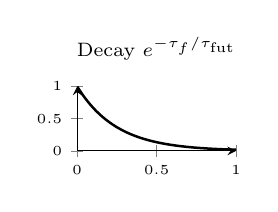
\begin{tikzpicture}
    \begin{axis}[width=3.6cm, height=2.4cm, xmin=0, xmax=1, ymin=0, ymax=1,
      xtick={0,0.5,1}, ytick={0,0.5,1},
      ticklabel style={font=\tiny}, every axis plot/.append style={line width=0.9pt},
      axis lines=left, title style={font=\scriptsize},
      title={\scriptsize Decay \(e^{-\tau_f/\tau_{\mathrm{fut}}}\)}]
      \addplot [domain=0:1, samples=200] {exp(-x/0.25)};
    \end{axis}
  \end{tikzpicture}
  };
  \node[tinycap, right=1mm of inset1] {gate on cumulative probability \(P(\tau_f)\)};
  \node[tinycap, right=1mm of inset2] {future decay with time constant \(\tau_{\mathrm{fut}}\)};

  % Badges (top-right alignment)
  \coordinate (badgeY)  at ($(fut.north east)+(0,12mm)$);
  \coordinate (badgeY2) at ($(badgeY)+(0,-6mm)$);

  \node[badge, anchor=south] (badge1) at ($(inset1.center |- badgeY)$)
    {$p(\tau_f)$: density [s$^{-1}$] \ \ $P(\tau_f)=\int_0^{\tau_f}\!p(u_f)\,du_f\in[0,1]$};
  \node[badge, anchor=south, yshift=-3mm] (badge2) at ($(inset2.center |- badgeY2)$)
    {$\kappa_w(t)$: [s$^{-1}$] \ \ $\displaystyle \gamma_b(t)=\int_0^{T_0}\!w(\tau_f,t)\,d\tau_f$};

  % Bottom row
  \node[title, below=16mm of sens] (title2) {Reduced surrogate (single effective retro-weight)};
  \node[chan, fill=gray!7, draw=black!70, below=6mm of title2] (collapse)
    {$\displaystyle \gamma_b(t)=\int_0^{T_0}\! w(\tau_f,t)\,d\tau_f$};
  \node[kern, fill=magenta!10, draw=magenta!60!black, right=of collapse, xshift=6mm] (Lb)
    {$\mathbf{D_{b}[\rho(t)]}$\\[-0.5mm]\scriptsize single jump w/ weight $\gamma_b(t)$};
  \node[kern, fill=blue!10, draw=blue!60!black, right=of Lb, xshift=6mm] (fwd)
    {$\mathbf{D_{\mathrm{fwd}}[\rho(t)]}$\\[-0.5mm]\scriptsize control (time-local)};

  \begin{scope}[on background layer]
    \draw[arr, preaction={draw=white, line width=3pt}]
      (fut.south) to[out=270, in=0] (collapse.east);
    \draw[arr, preaction={draw=white, line width=3pt}] (collapse) -- (Lb);
    \draw[arr, preaction={draw=white, line width=3pt}] (Lb) -- (fwd);
  \end{scope}

  \node[tinycap, below=4mm of Lb]
    {collapse of the continuum $\{L_b(\tau_f,t)\}_{\tau_f\in[0,T_0]}$ to a single effective jump $L_b(t)$ with \emph{weight} $\gamma_b(t)$ (see SI)};

  % ===== TIGHT BOUNDING BOX (captures all pictorial elements safely) =====
  % Fit node around ALL elements you want included in the cropping box:
  \begin{scope}[on background layer]
    \node[fit=(mem)(sens)(fut)(gate)(inset1)(inset2)(badge1)(badge2)(collapse)(Lb)(fwd),
          inner sep=2mm, name=CRIfit]{};
    \path[use as bounding box] (CRIfit.north west) rectangle (CRIfit.south east);
  \end{scope}

  \end{tikzpicture}
  \end{adjustbox}

  % CAPTION stays inside the sidewaysfigure float, directly under the graphic:
  \caption{%
    \textsc{CRI kernel interactions and reduced surrogate. The full nonlocal generator comprises a memory dissipator $D_{\mathrm{mem}}$ (past kernel $K(s)$), a Markovian sensory channel $D_{\mathrm{sens}}$, and a future-indexed dissipator $D_{\mathrm{future}}[\rho] =\int_{0}^{T_0} w(\tau_f,t)\,\mathcal{D}\!\big[L_b(\tau_f,t)\big]\rho\,d\tau_f$. The retro-weight $w(\tau_f,t)=\kappa_w(t)\,G\!\big(P(\tau_f)-p_0(a(t))\big)\,e^{-\tau_f/\tau_{\mathrm{fut}}}$ combines a dimensionless gate $G$ driven by the cumulative probability $P(\tau_f)=\int_{0}^{\tau_f}p(u_f)\,du_f$ (with density $p(\tau_f)$ in s$^{-1}$) and a short retro-decay with time constant $\tau_{\mathrm{fut}}$; $\kappa_w(t)$ has units s$^{-1}$. Collapsing the continuum yields the reduced surrogate with a single effective jump $\mathbf{D_{b}[\rho(t)]}\equiv \gamma_b(t)\,\mathcal{D}[L_b]\rho(t)$ at \emph{weight} $\gamma_b(t)=\int_{0}^{T_0} w(\tau_f,t)\,d\tau_f$ (dimensionless), optionally paired with a time-local forward control $D_{\mathrm{fwd}}$ for identifiability/ablation (not an extra physical channel in the full nonlocal model). The construction is GKSL-admissible (completely positive and trace preserving) and, since weights are predictive (not postselected), compatible with no-signalling-in-time (NSIT); see Eq.~\eqref{eq:cri-master} for the full model and Eq.~\eqref{eq:reduced-surrogate} for the surrogate.}
  }
  \label{fig:cri-sideways}
\end{sidewaysfigure}
